\subsection{Experiment \rnum{1}: Model training and Reconstruction}

\begin{table}[!htbp]
    \centering
    \small
    \setlength{\tabcolsep}{10pt}
    \begin{tabular}{l S[table-format=1.3e-2] S[table-format=2.1] S[table-format=1.3e-2] S[table-format=1.1e-3]}
        \toprule
        \rowcolor{gray!20}
        \textbf{Metric} & {\textbf{AE}} & {\textbf{$\beta$-VAE}} & {\textbf{CAE}} & {\textbf{$\beta$-CVAE}} \\
        \midrule
        Best Train loss & 1.300e-6 & 21.3 & 1.370e-4 & 4.5e-3 \\
        \rowcolor{gray!10} Best Validation loss & 1.300e-6 & 21.3 & 5.400e-5 & 4.4e-3 \\
        Epochs before stop & 6 & 20 & 15 & 15 \\
        \rowcolor{gray!10} Model Sizes & {\SI{10.240}{\giga\byte}} & {\SI{11.200}{\giga\byte}} & {\textbf{\SI{0.18}{\mega\byte}}} & {\textbf{\SI{47.06}{\mega\byte}}} \\
        Inference speed F32 (\si{\milli\second}) & 1.658 & 654.14 & 267.31 & 979.52 \\
        \rowcolor{gray!10} Inference speed F16 (\si{\milli\second}) & 1.875 & 6.31 & 5.671 & 1.857 \\
        \bottomrule
    \end{tabular}
    \caption{Comparison of Autoencoder Performance}
    \label{tab:modelresinfo}
    \smallskip
    \small{*The reconstruction error is the sum of all reconstruction errors across all batches.}
\end{table}


\begin{figure}[!h]
    \centering
    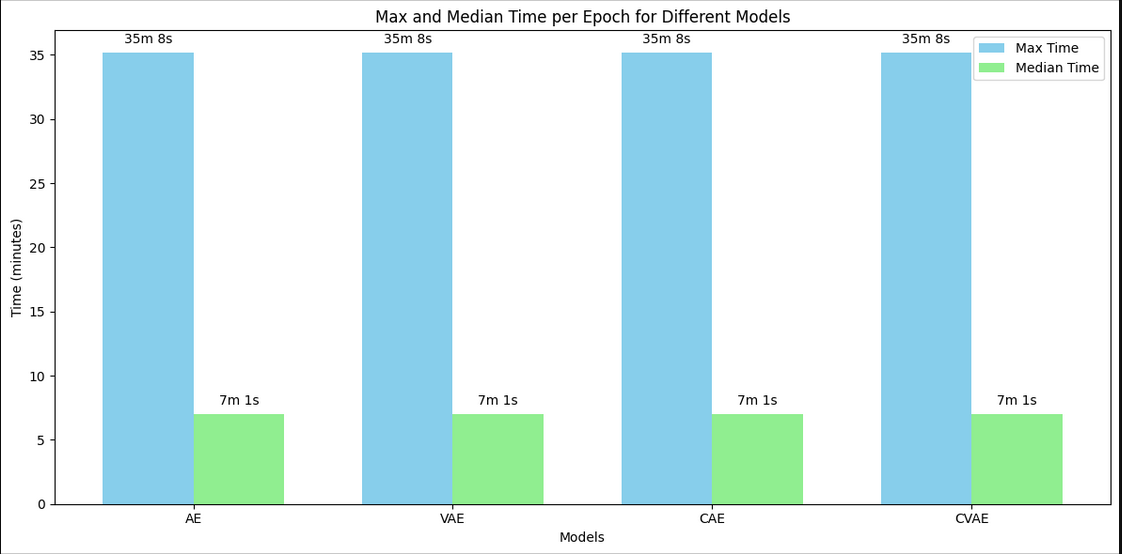
\includegraphics[scale=0.35]{figures/time.png}
    \caption{Comparison between Maximum and mediant amount of time spent per epoch}
    \label{fig:traintimes}
\end{figure}

\clearpage

\subsubsection{Train and Validation Losses}

\begin{figure}[!h]
  \centering
  \begin{subfigure}[t]{.6\textwidth}
    \centering
    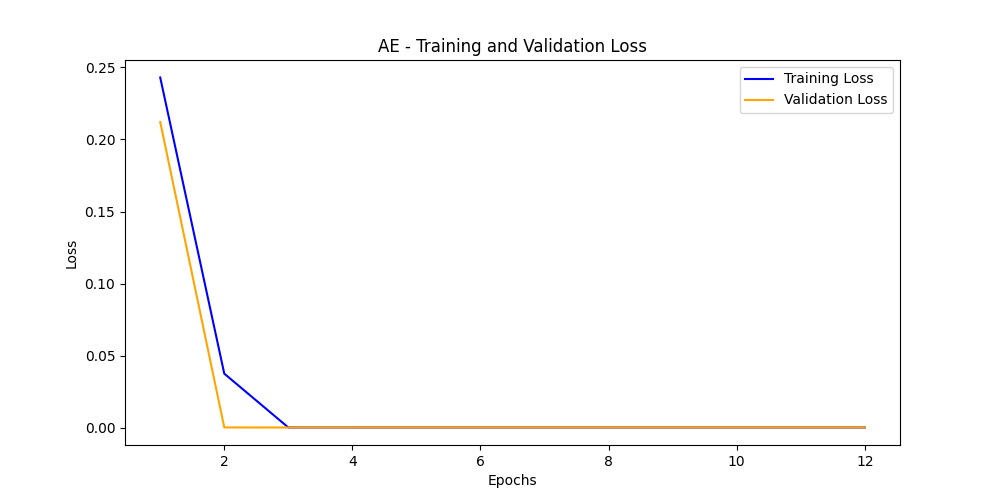
\includegraphics[width=\linewidth]{figures/losses/ae.png}
    \caption{AE}
  \end{subfigure}
  \hfill
  \begin{subfigure}[t]{.6\textwidth}
    \centering
    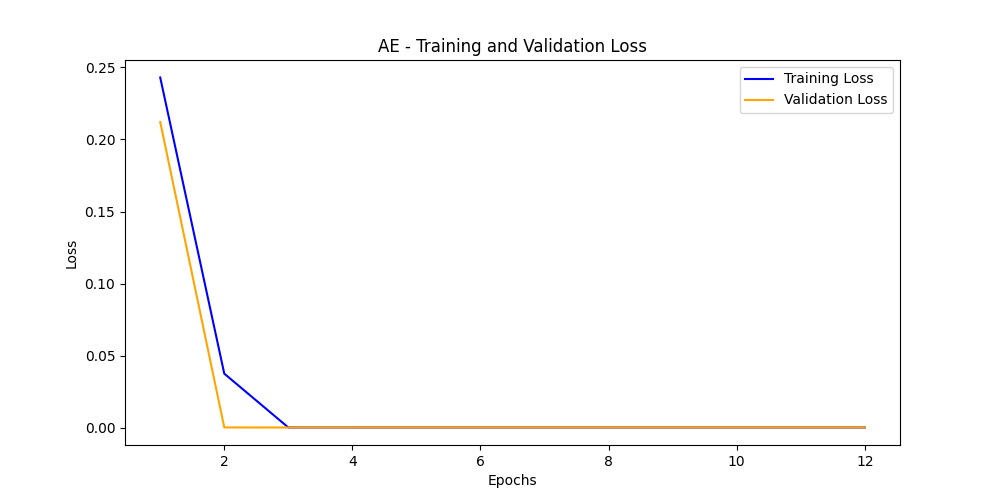
\includegraphics[width=\linewidth]{figures/losses/ae.png}
    \caption{$\beta$-VAE}
  \end{subfigure}
  
  \vspace{1cm}
  
  \begin{subfigure}[t]{.6\textwidth}
    \centering
    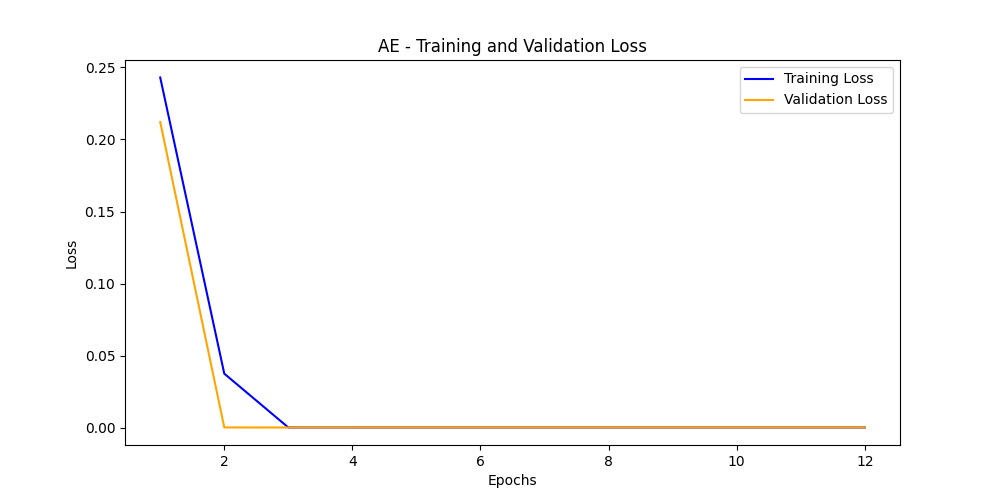
\includegraphics[width=\linewidth]{figures/losses/ae.png}
    \caption{CAE}
  \end{subfigure}
  \hfill
  \begin{subfigure}[t]{.6\textwidth}
    \centering
    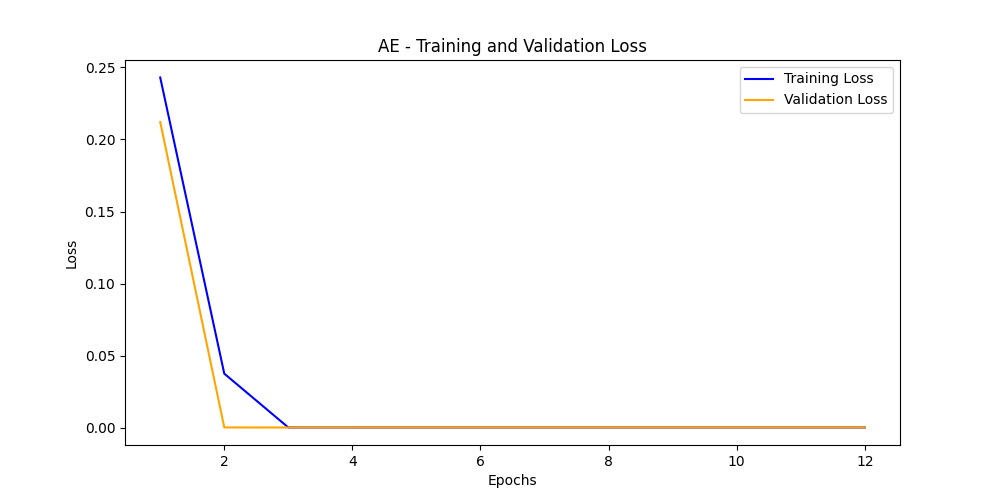
\includegraphics[width=\linewidth]{figures/losses/ae.png}
    \caption{$\beta$-CVAE}
  \end{subfigure}
  \label{fig:losses}
  \caption{Train and Validation Loss over Time}
\end{figure}

\clearpage

\subsubsection{Heatmap Reconstruction Comparison}

\begin{figure}[!h]
\centering
% Row 0 (Image Names)
\begin{subfigure}{0.33\textwidth}
\centering
2019-04-15 03:17:35
\end{subfigure}%
\hfill
\begin{subfigure}{0.33\textwidth}
\centering
2019-04-15 03:17:50
\end{subfigure}%
\hfill
\begin{subfigure}{0.33\textwidth}
\centering
2019-04-15 03:17:55
\end{subfigure}

    \vspace{1em}
    
    % Row 1 (Original)
    \begin{subfigure}{0.33\textwidth}
        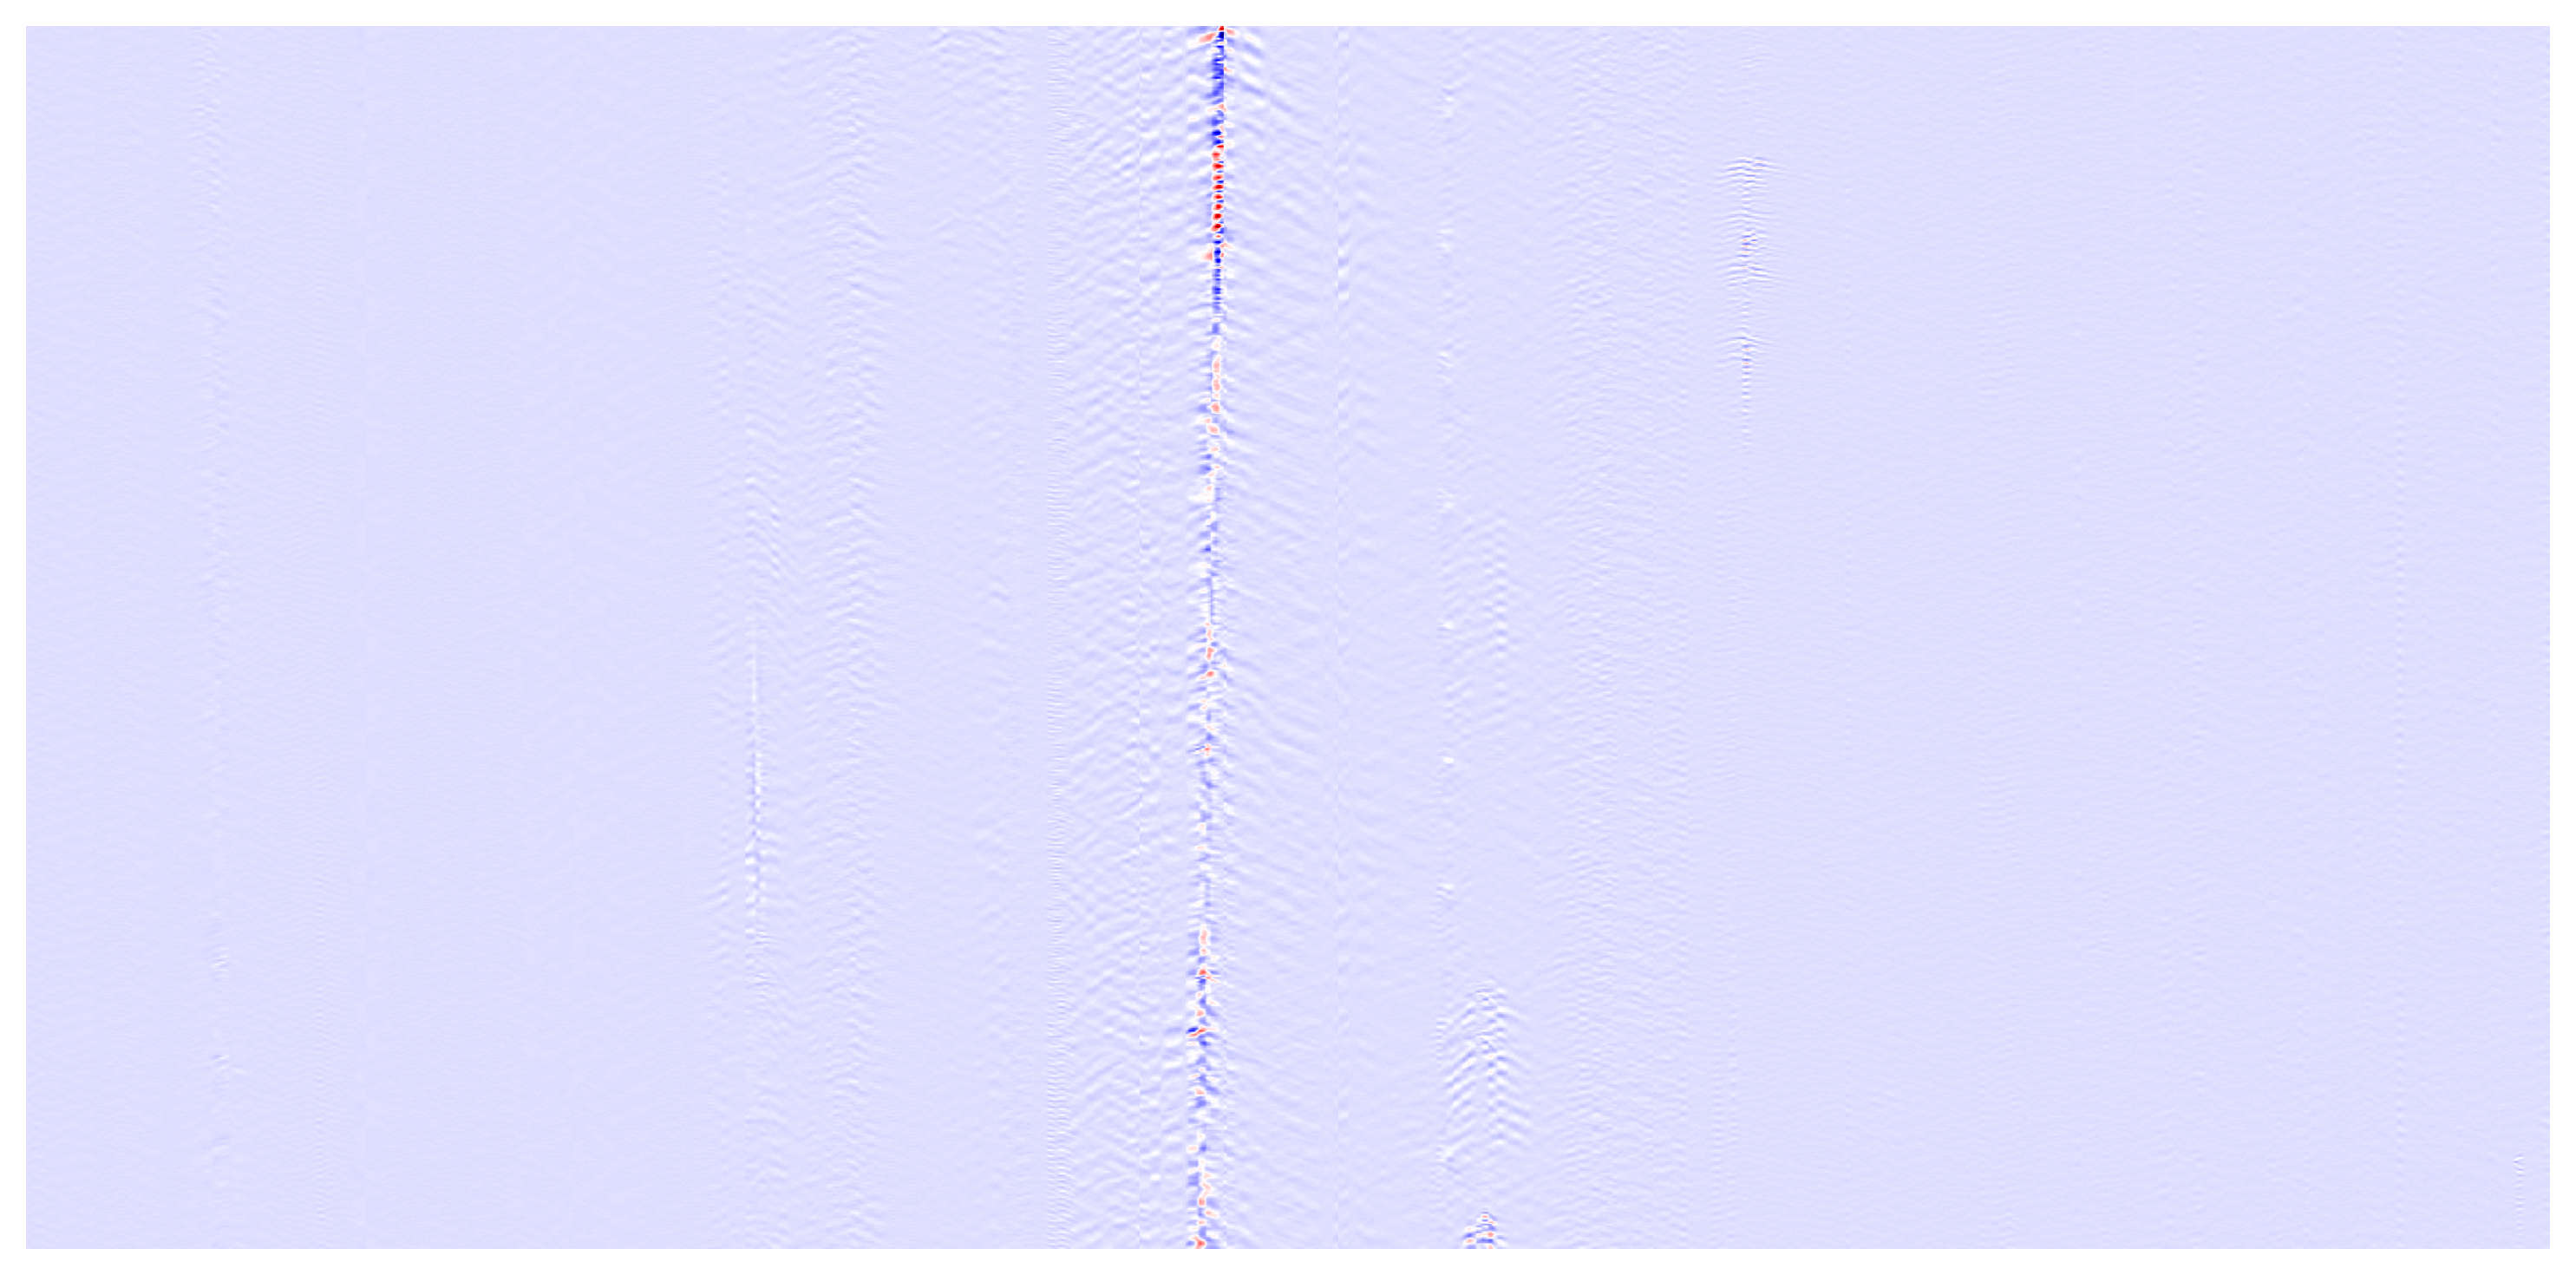
\includegraphics[width=\textwidth]{figures/anomalies/before/20190415_031735.png}
    \end{subfigure}%
    \hfill
    \begin{subfigure}{0.33\textwidth}
        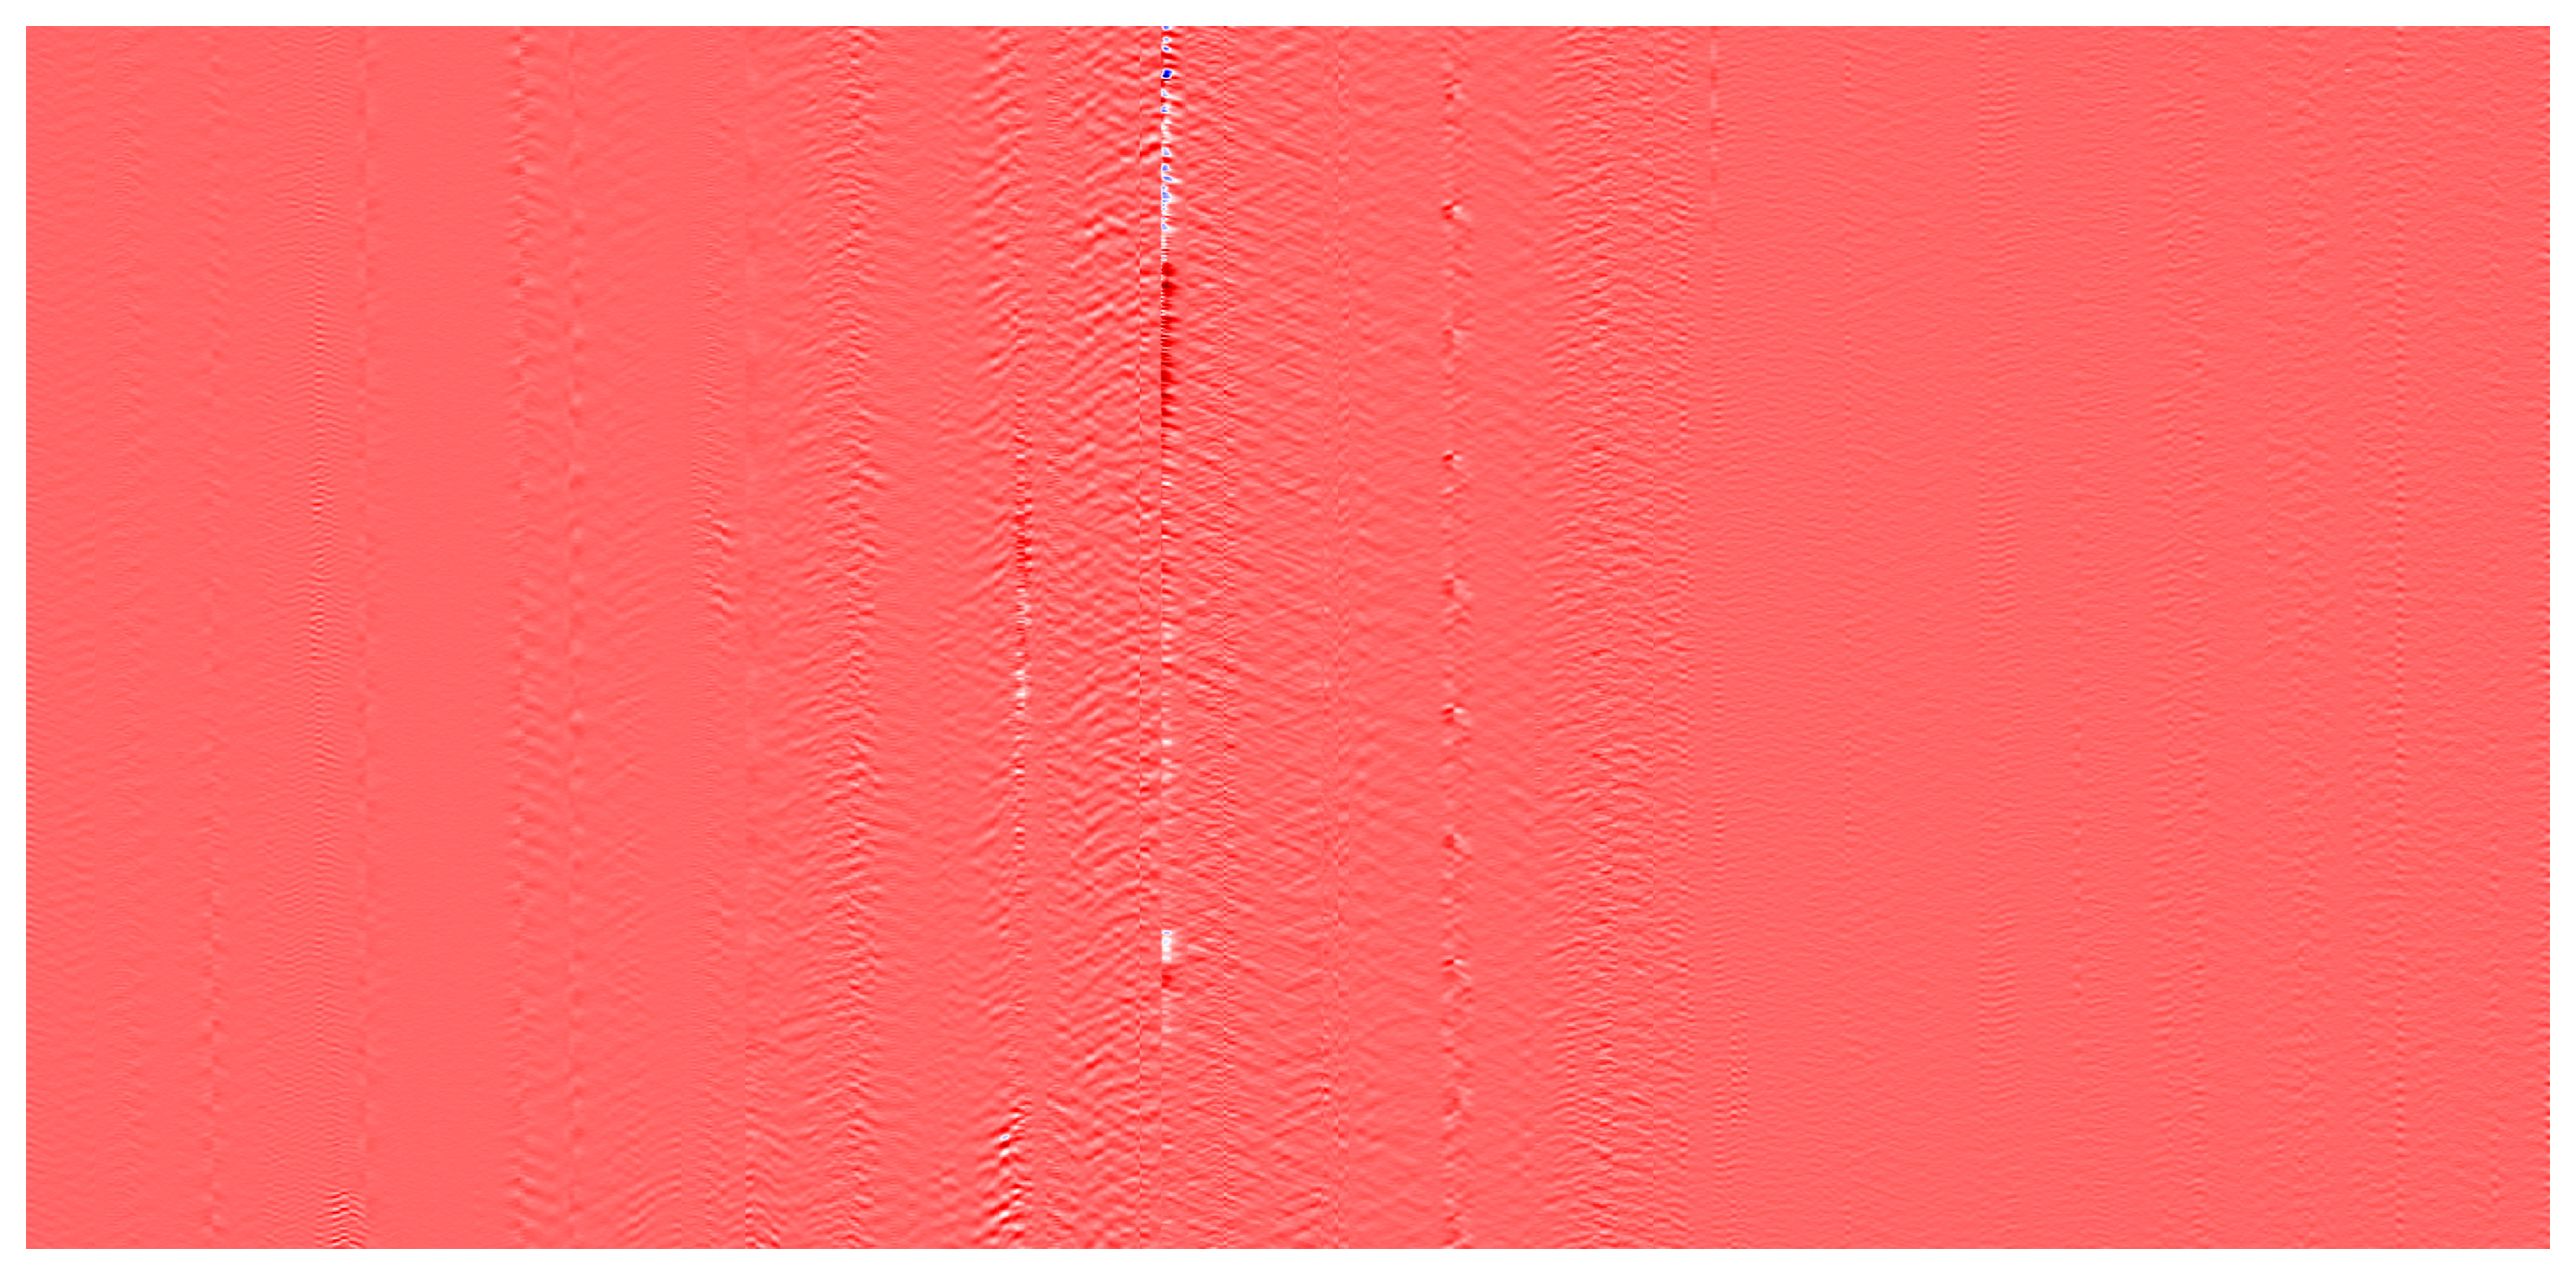
\includegraphics[width=\textwidth]{figures/anomalies/before/20190415_031750.png}
    \end{subfigure}%
    \hfill
    \begin{subfigure}{0.33\textwidth}
        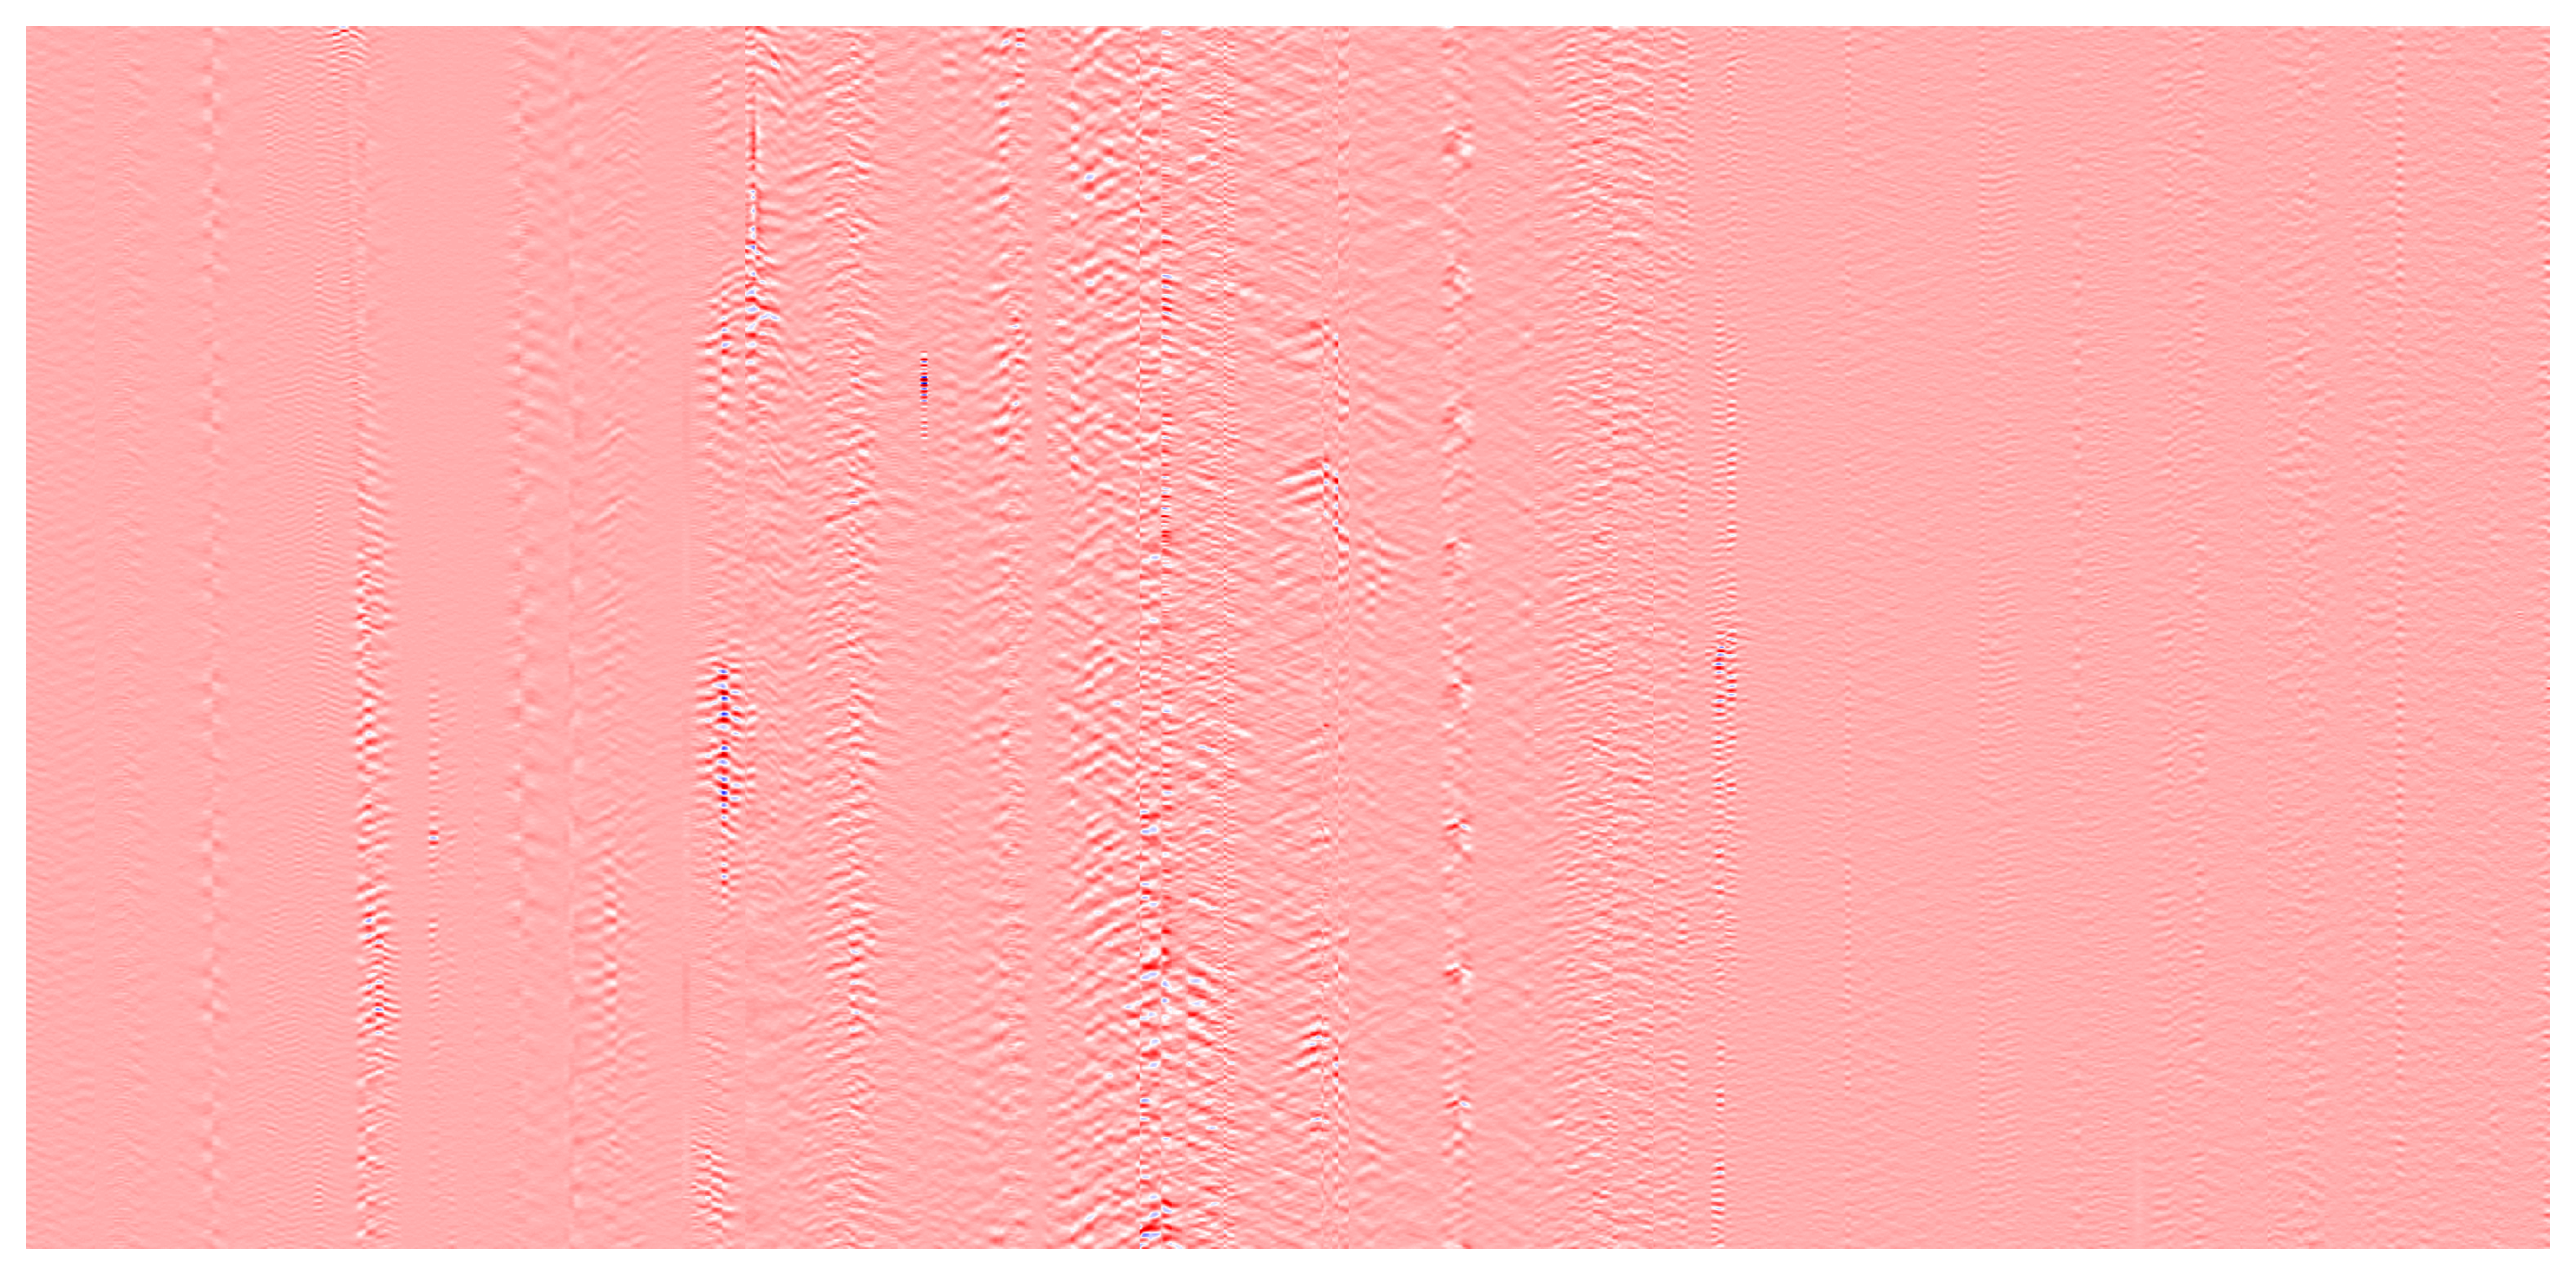
\includegraphics[width=\textwidth]{figures/anomalies/before/20190415_031755.png}
    \end{subfigure}
    
    \vspace{1em}
    
    % Row 2 (Model 1)
    \begin{subfigure}{0.33\textwidth}
        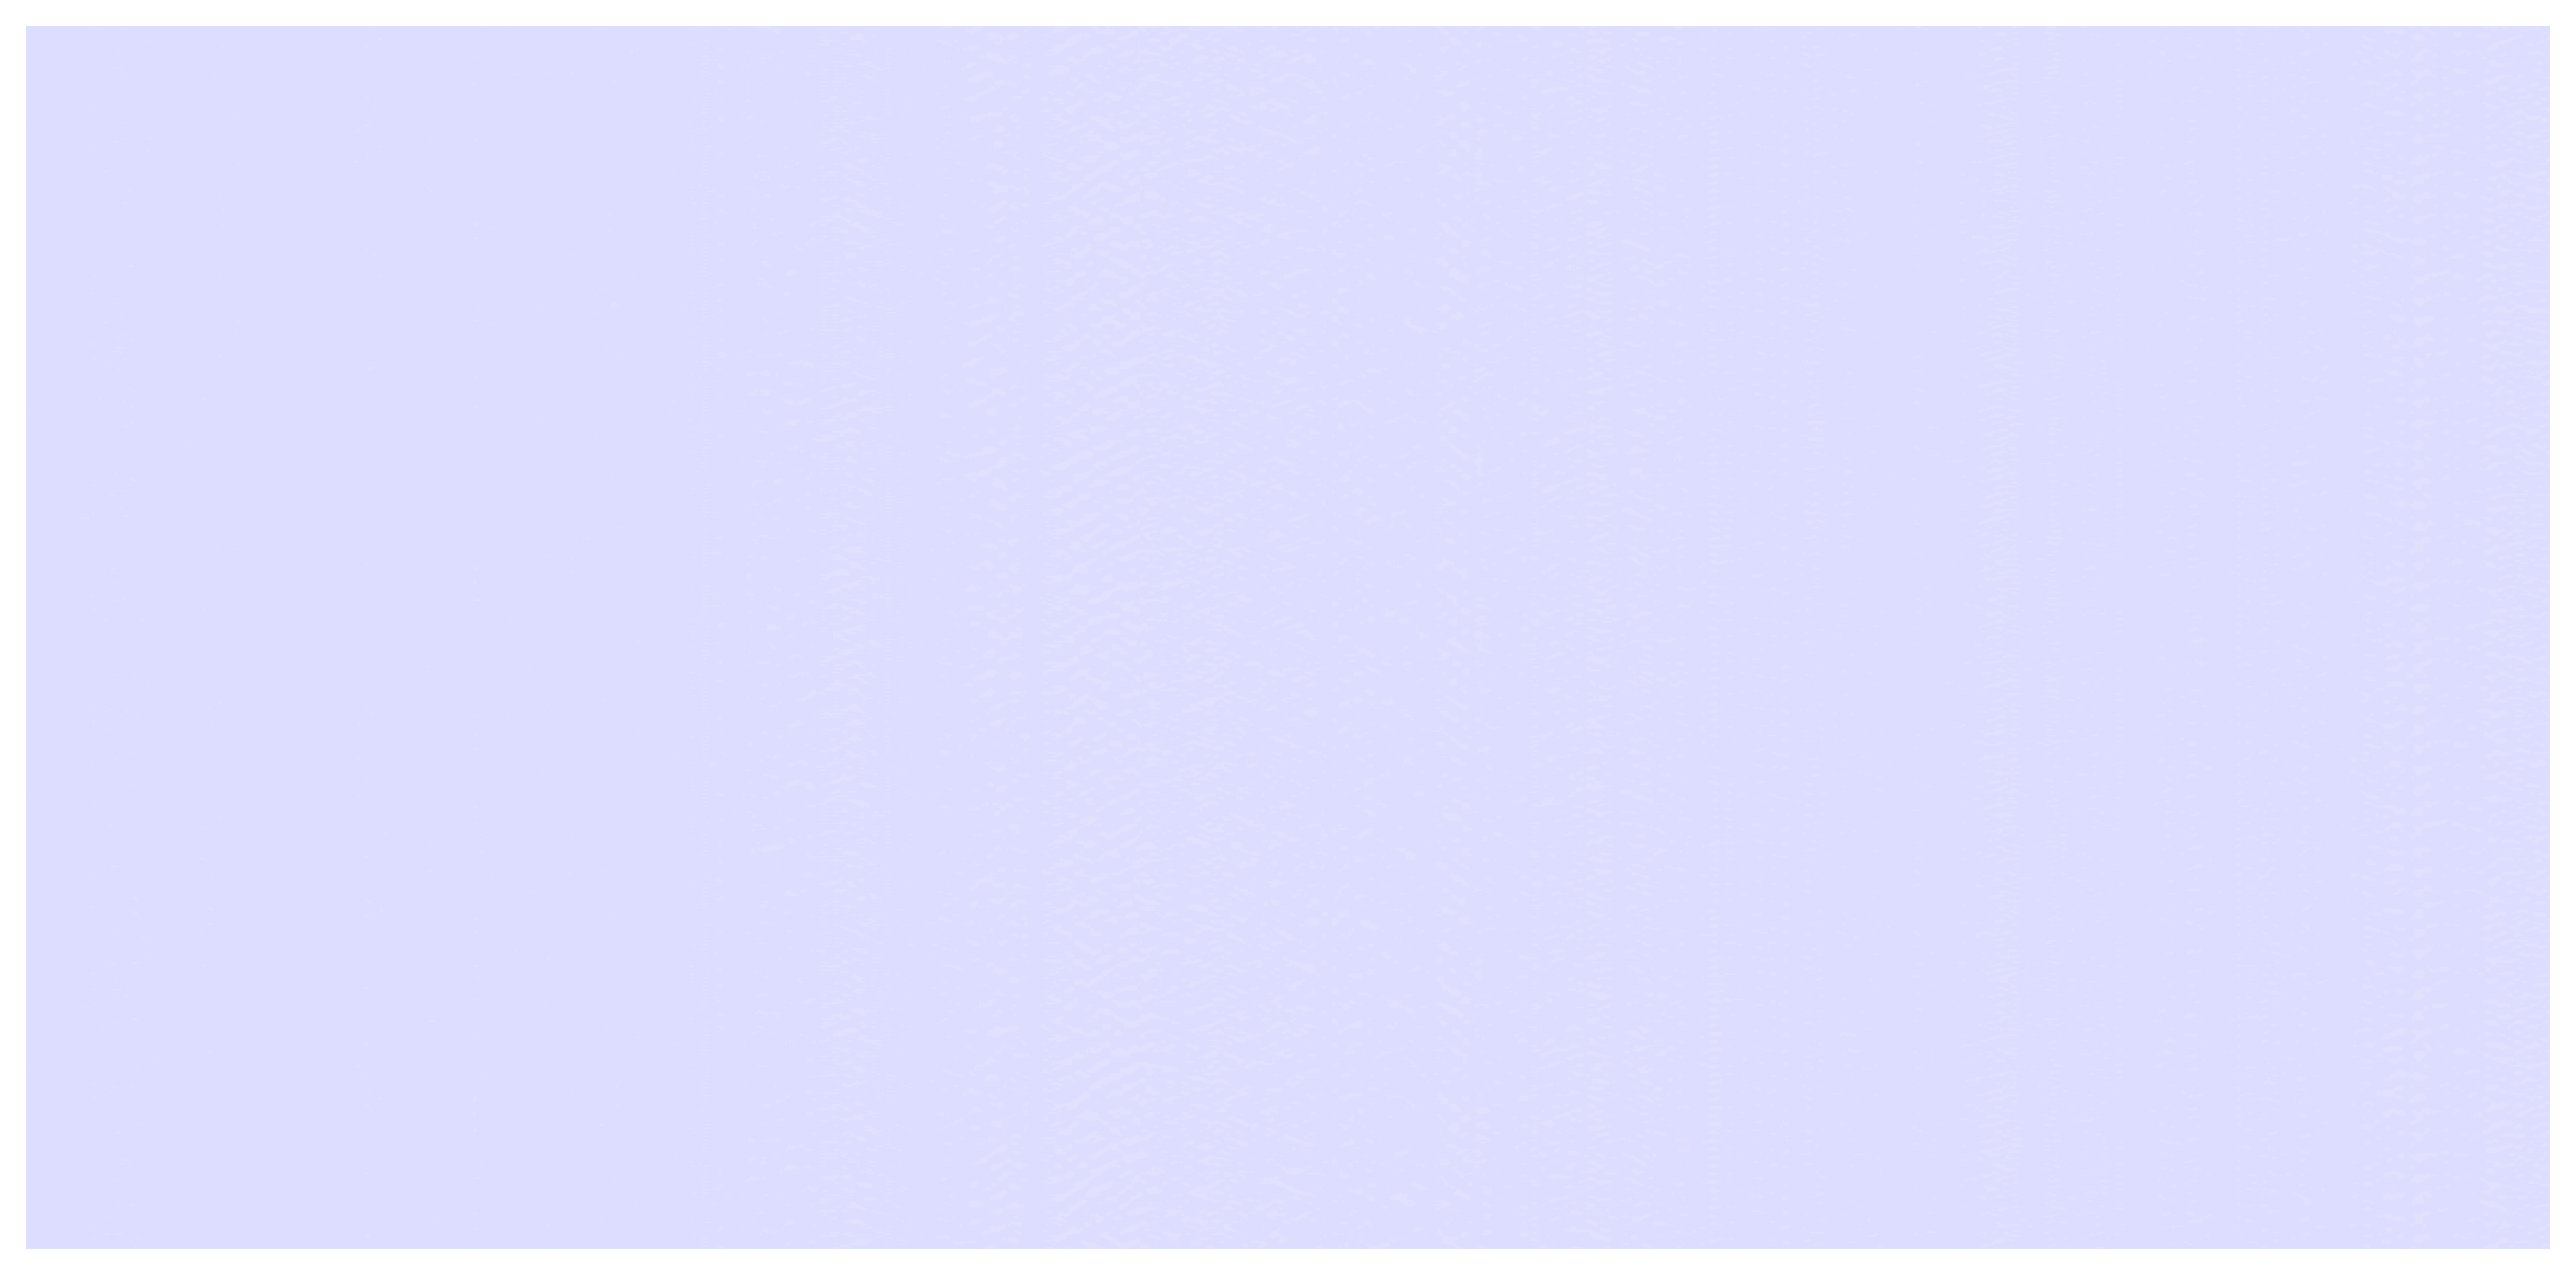
\includegraphics[width=\textwidth]{figures/anomalies/ae/20190415_031735.png}
    \end{subfigure}%
    \hfill
    \begin{subfigure}{0.33\textwidth}
        
\includegraphics[width=\textwidth]{figures/anomalies/ae/20190415_031750.png}
    \end{subfigure}%
    \hfill
    \begin{subfigure}{0.33\textwidth}
        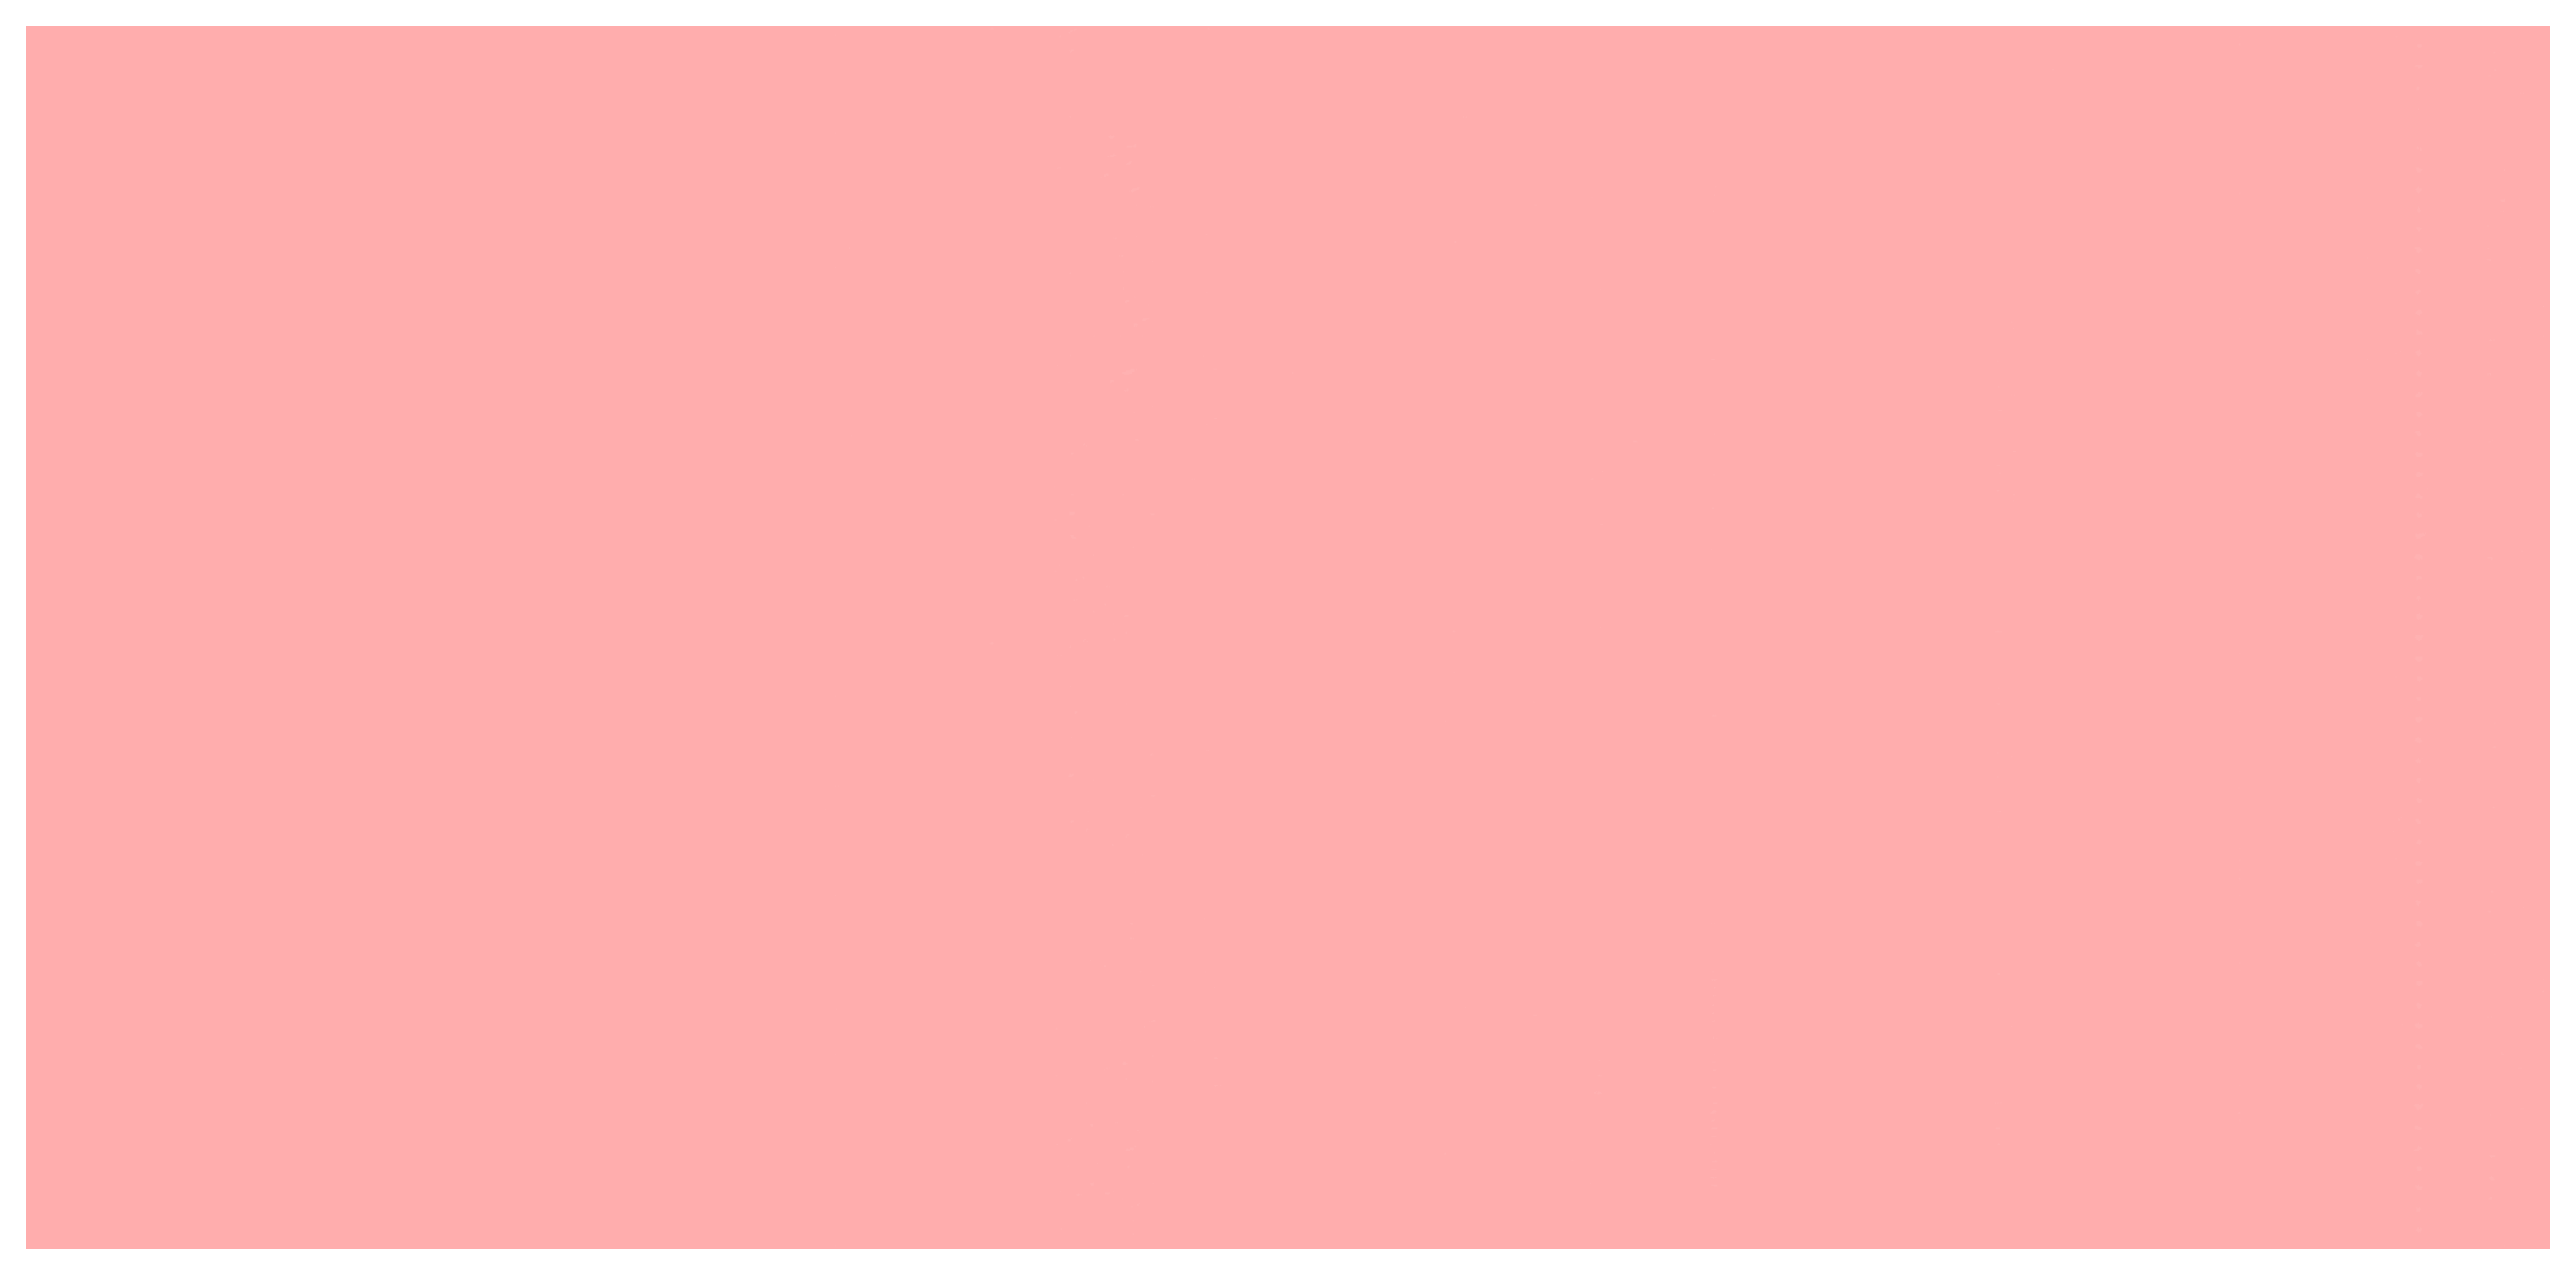
\includegraphics[width=\textwidth]{figures/anomalies/ae/20190415_031755.png}
    \end{subfigure}
    
    \vspace{1em}
    
    
    % Row 4 (Model 3)
    \begin{subfigure}{0.33\textwidth}
        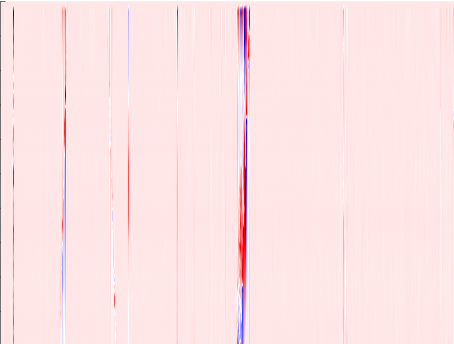
\includegraphics[width=\textwidth]{figures/test.png}
    \end{subfigure}%
    \hfill
    \begin{subfigure}{0.33\textwidth}
        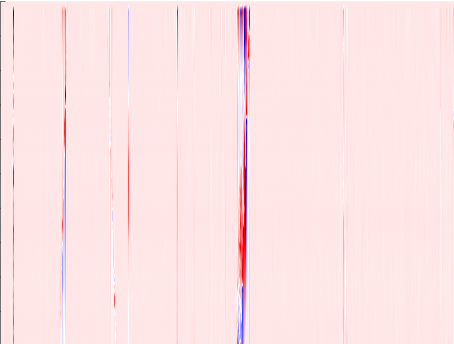
\includegraphics[width=\textwidth]{figures/test.png}
    \end{subfigure}%
    \hfill
    \begin{subfigure}{0.33\textwidth}
        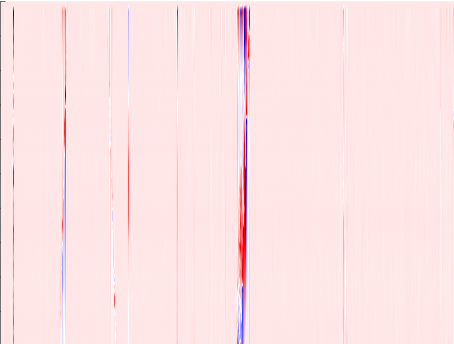
\includegraphics[width=\textwidth]{figures/test.png}
    \end{subfigure}


    \vspace{1em}
    
    % Row 3 (Model 2)
    \begin{subfigure}{0.33\textwidth}
        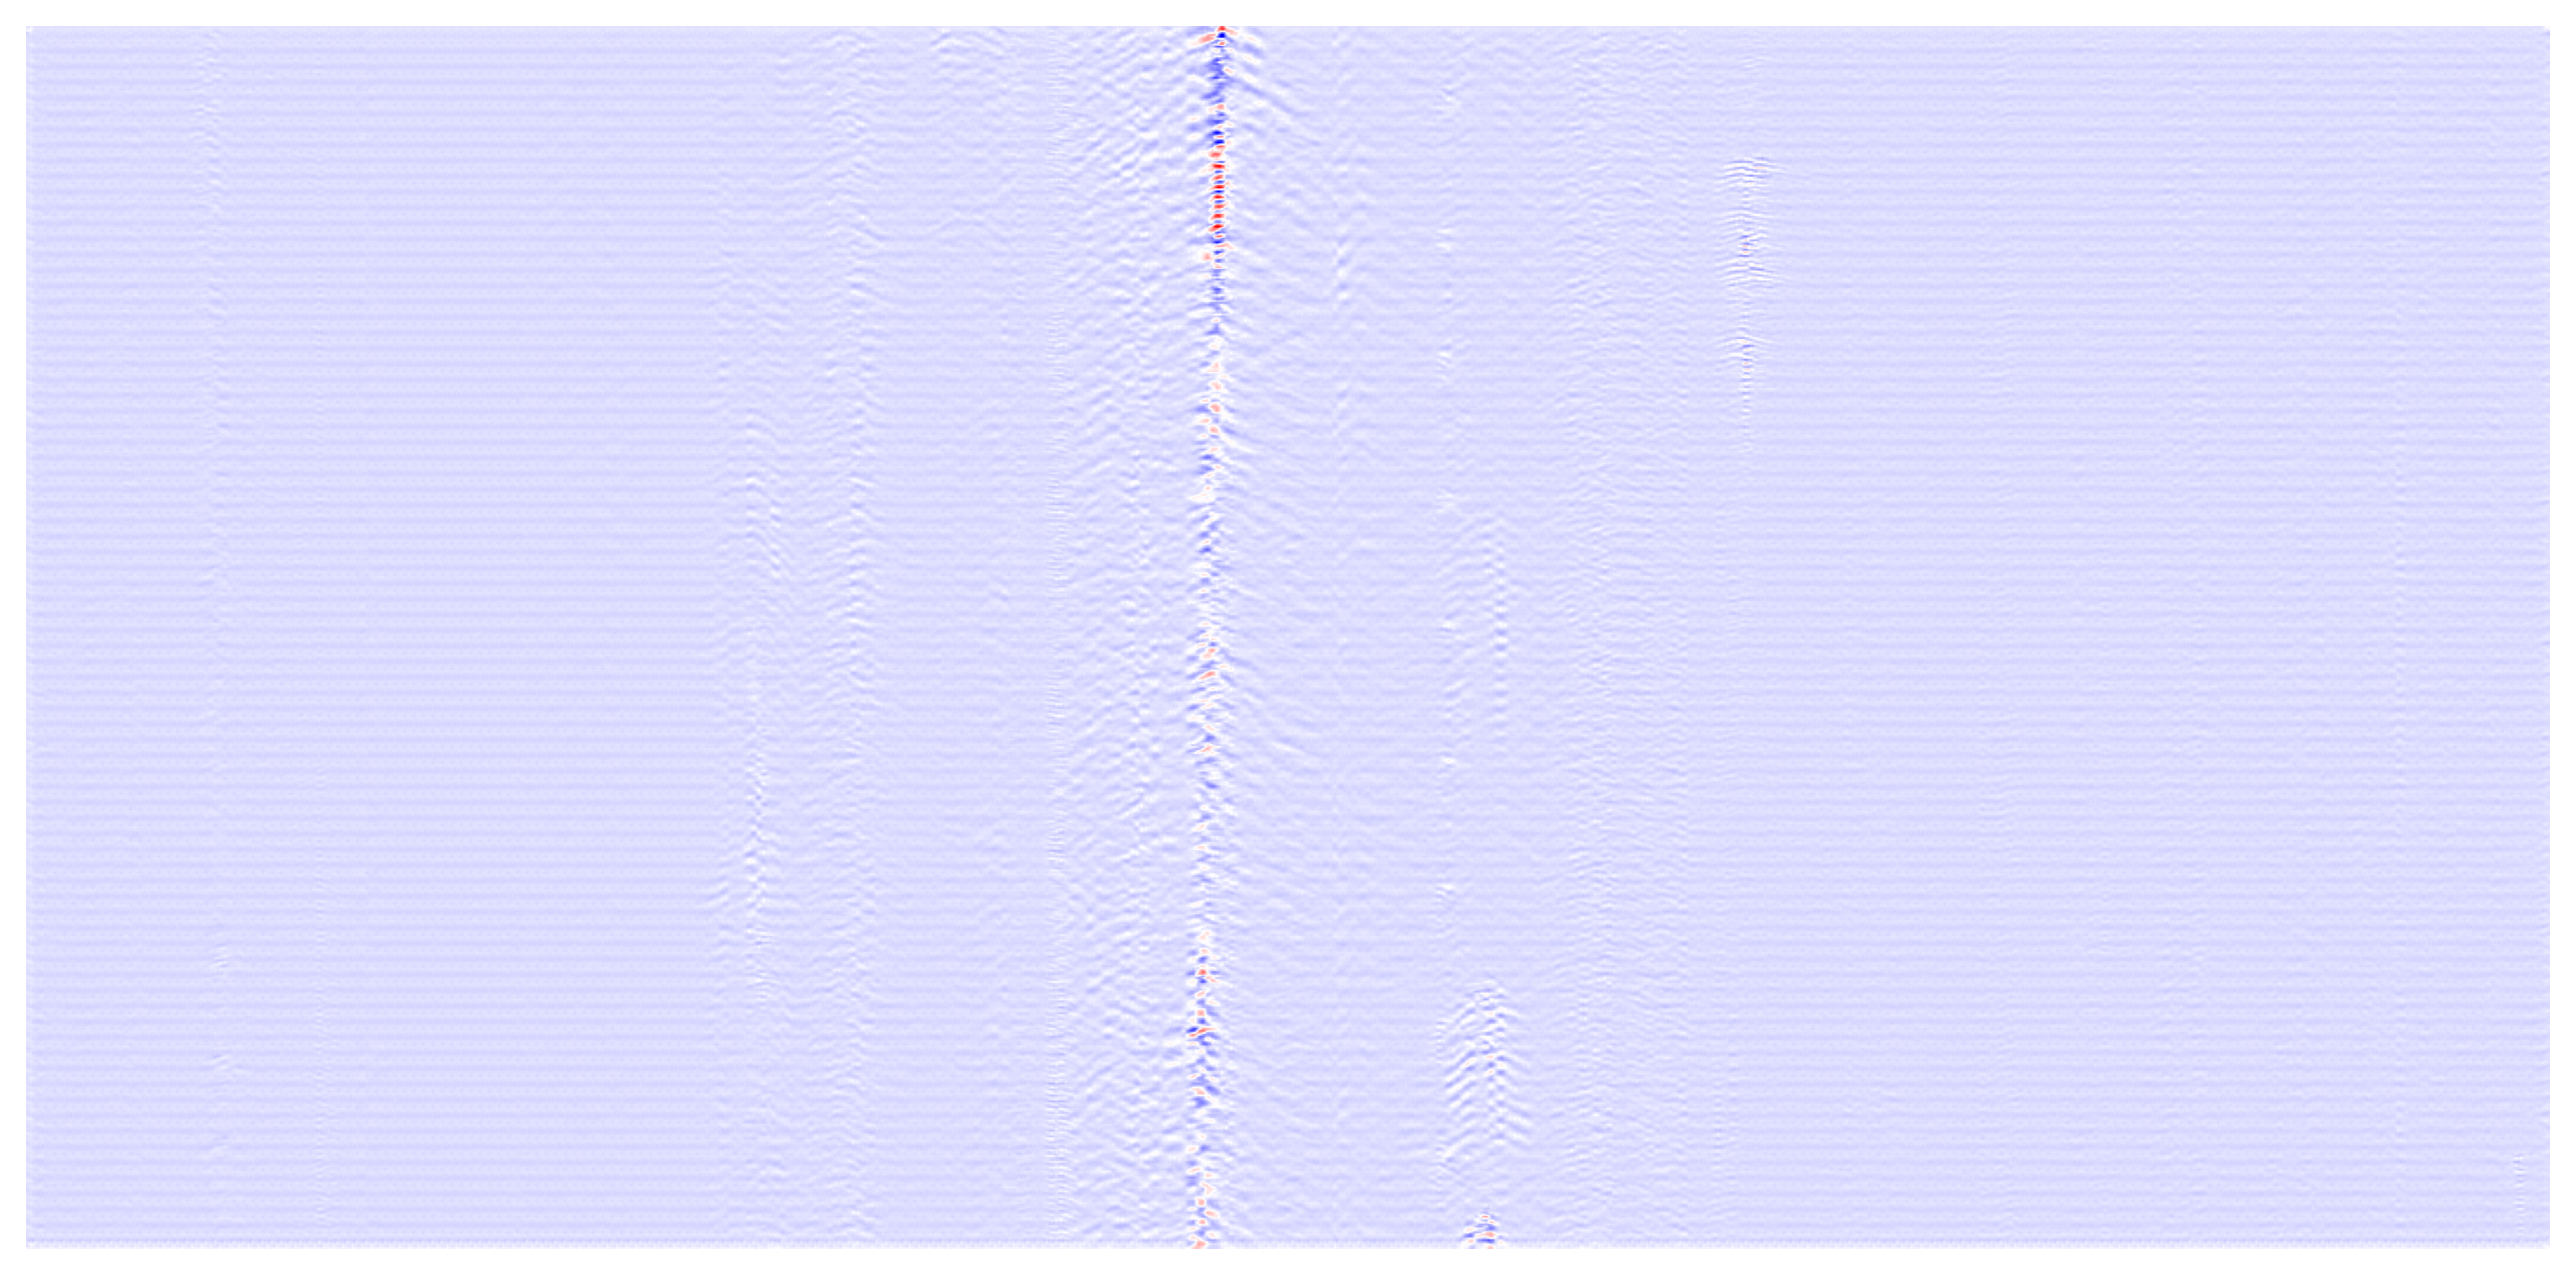
\includegraphics[width=\textwidth]{figures/anomalies/cae/20190415_031735.png}
    \end{subfigure}%
    \hfill
    \begin{subfigure}{0.33\textwidth}
        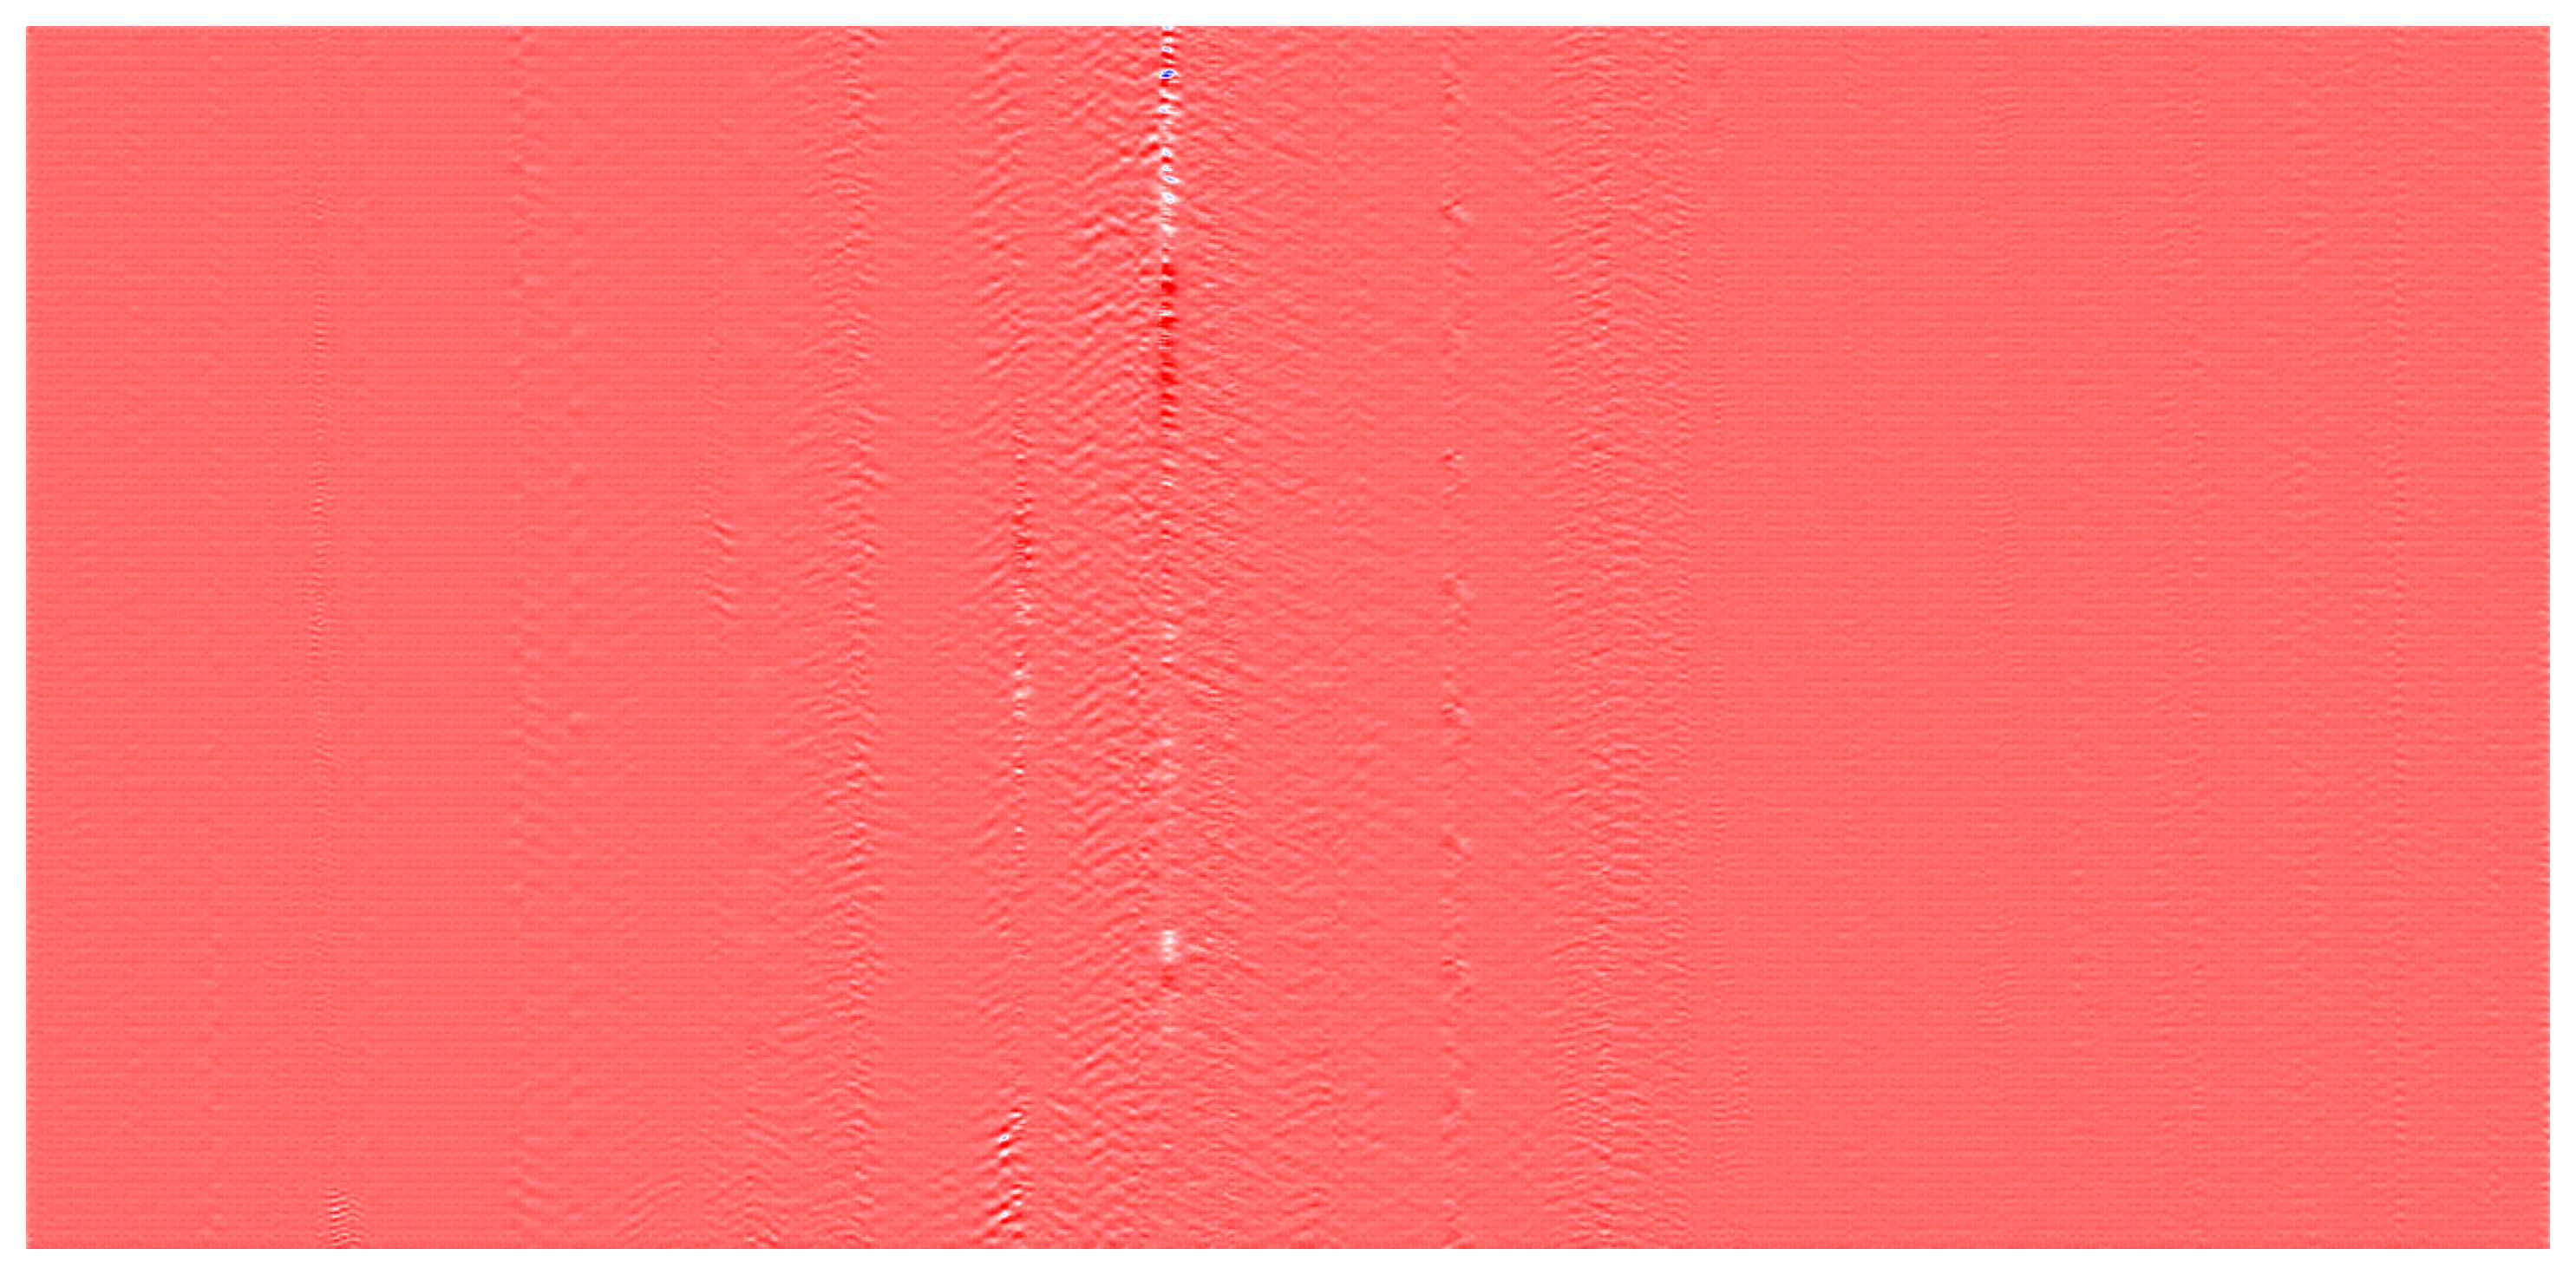
\includegraphics[width=\textwidth]{figures/anomalies/cae/20190415_031750.png}
    \end{subfigure}%
    \hfill
    \begin{subfigure}{0.33\textwidth}
        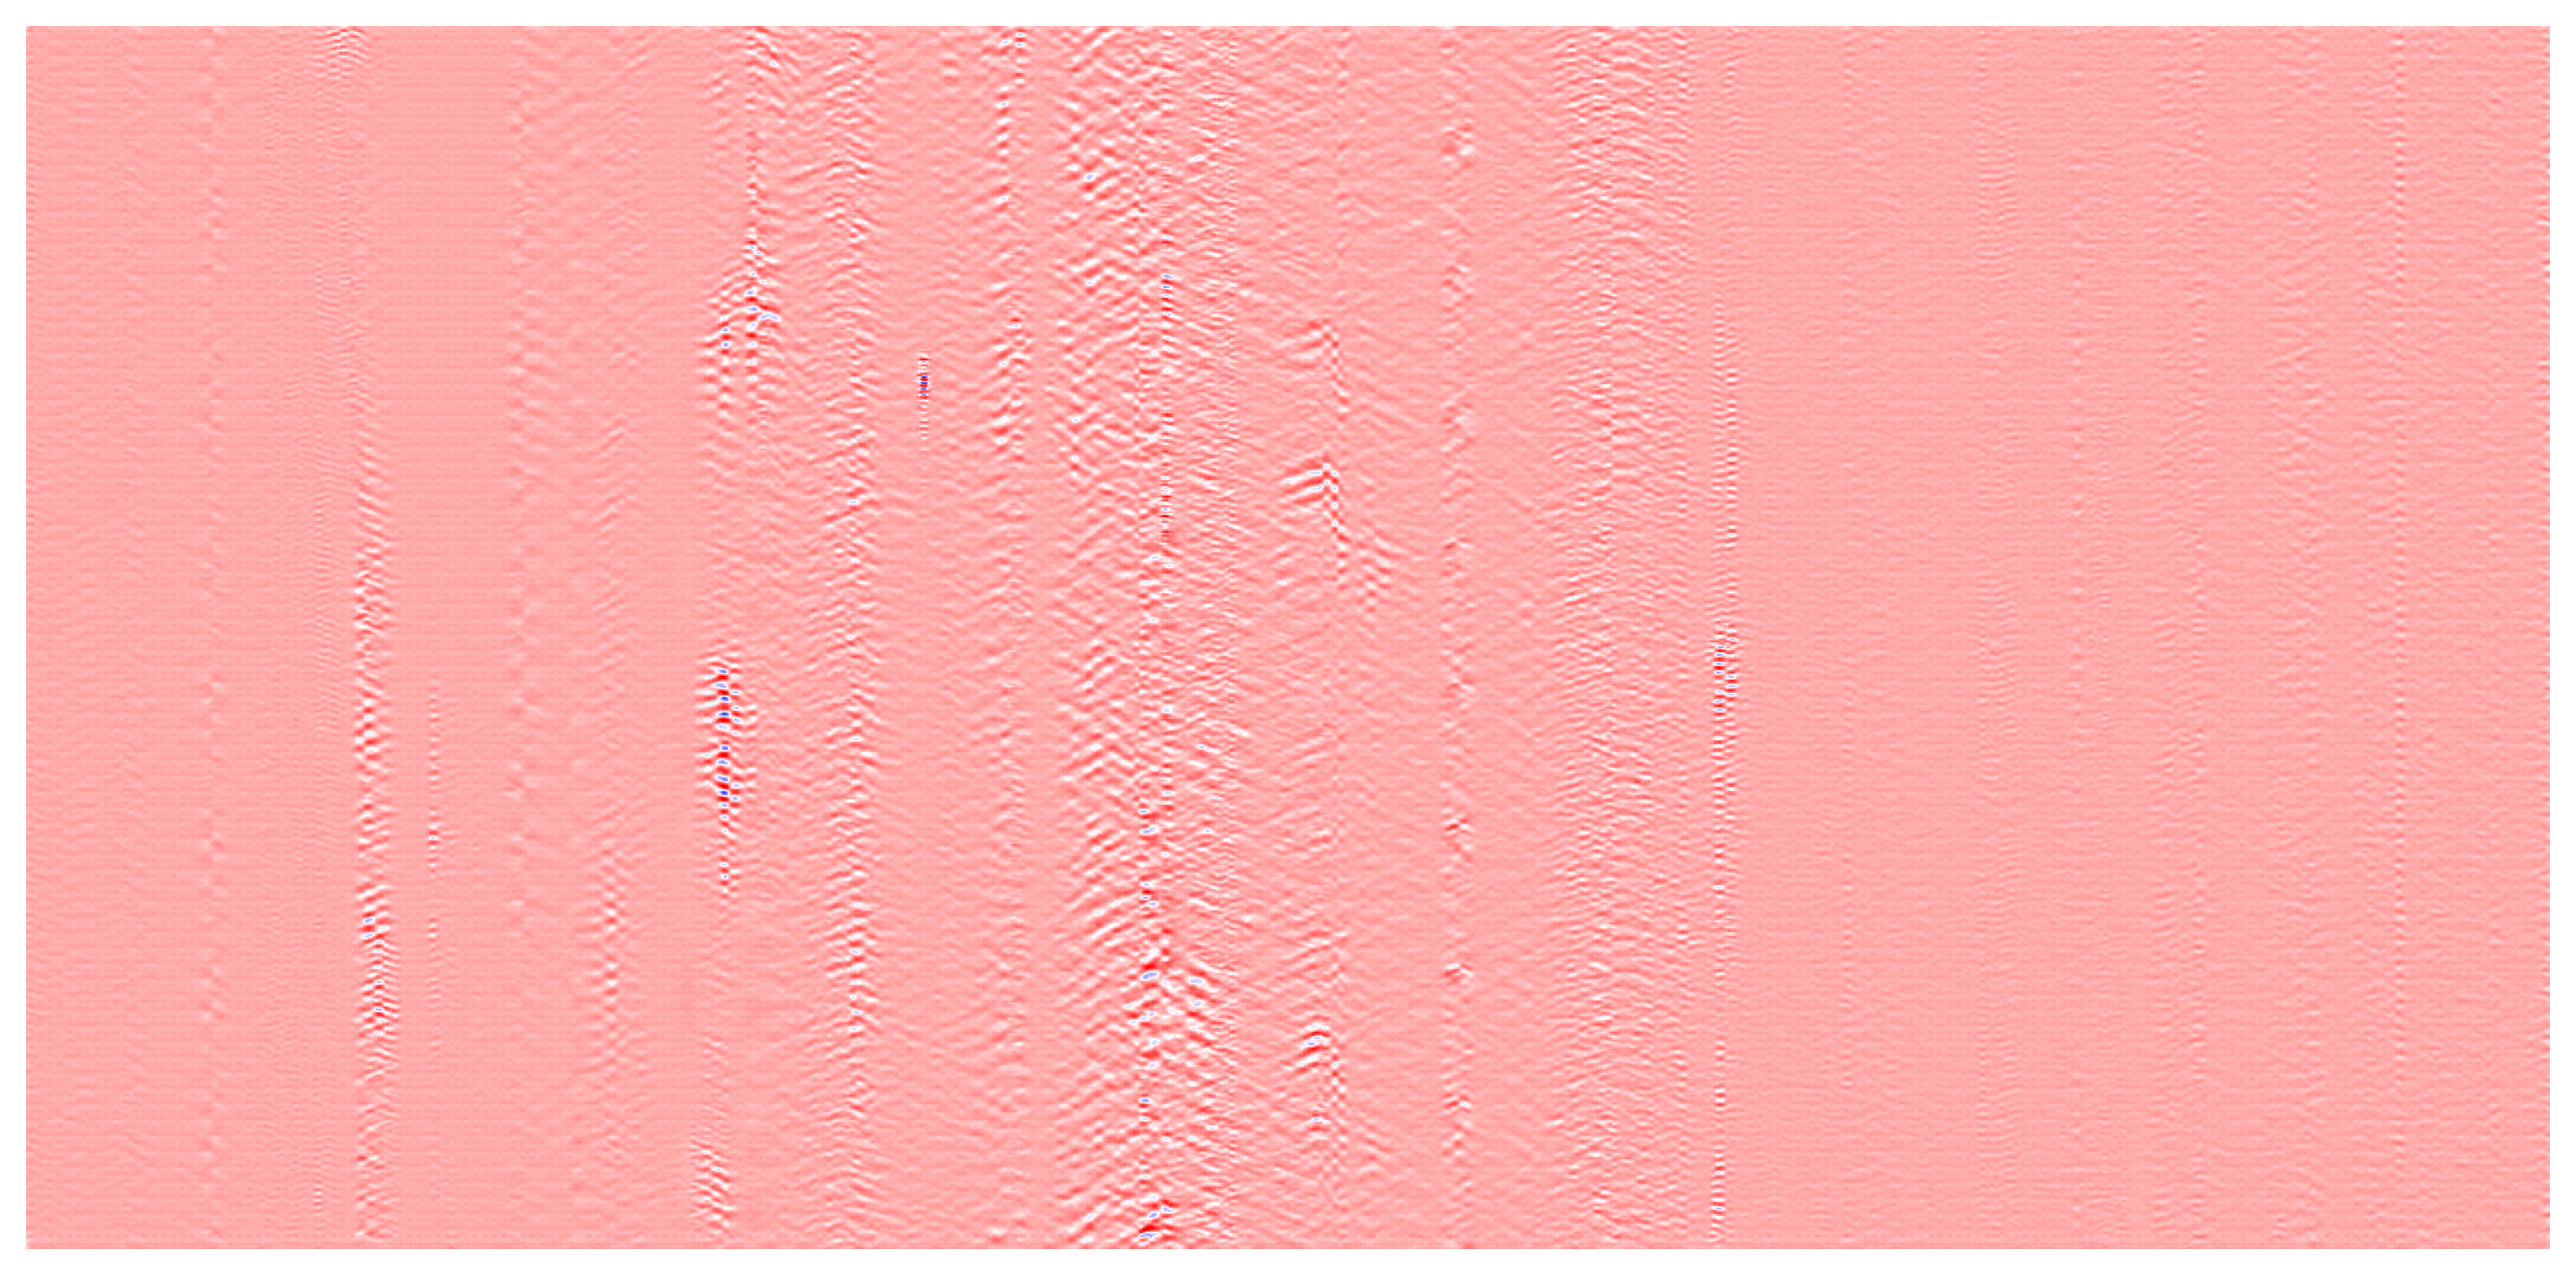
\includegraphics[width=\textwidth]{figures/anomalies/cae/20190415_031755.png}
    \end{subfigure}
    
    
    \vspace{1em}
    
    % Row 5 (Model 4)
    \begin{subfigure}{0.33\textwidth}
        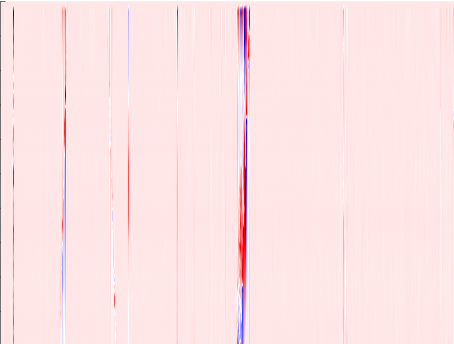
\includegraphics[width=\textwidth]{figures/test.png}
    \end{subfigure}%
    \hfill
    \begin{subfigure}{0.33\textwidth}
        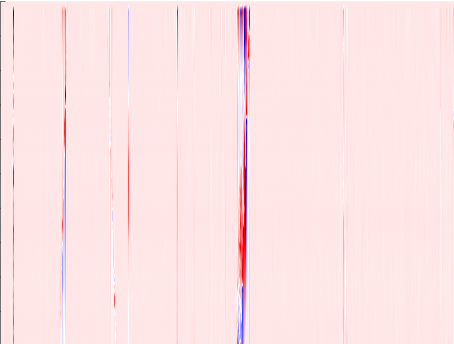
\includegraphics[width=\textwidth]{figures/test.png}
    \end{subfigure}%
    \hfill
    \begin{subfigure}{0.33\textwidth}
        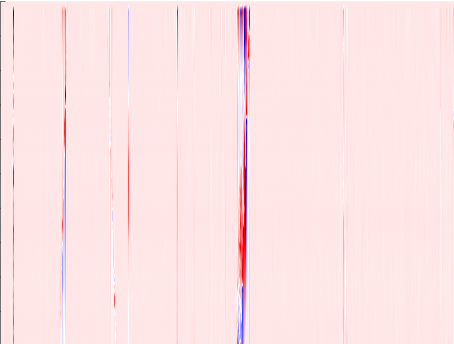
\includegraphics[width=\textwidth]{figures/test.png}
    \end{subfigure}
    
    \caption{Comparison of original heatmaps and their reconstructions by different mdoels. The top row consist of original \acrshort{das} heatmaps, followed by reconstructions produced by: AE, $\beta$-VAE, CAE and $\beta$-CVAE}
    \label{fig:aereconstruct}
\end{figure}
